\chapter{तंत्रिका-तंत्रों का संगठन}\label{ch:b3:nervous-systems}

किसी जेलीमीन के पास बिना किसी केंद्र वाले किसी जाल में कुछ हज़ार
न्यूरॉन हैं और वह तैर सकती है, खा सकती है और खुद को सीधा कर सकती है।
किसी ऑक्टोपस के पास आधा अरब हैं, जिनके दो-तिहाई उसकी भुजाओं में हैं,
और हर भुजा कोई ऐसी समस्या हल कर सकती है जिसकी ख़बर मस्तिष्क को दी ही
नहीं गई। आपके पास छियासी अरब हैं, जो सौ खरब तंत्रिका-संधियों से जुड़े
हैं और बीस वाट पर चलते हैं --- आपके द्रव्यमान के दो प्रतिशत के लिए
आपकी ऊर्जा का पाँचवाँ भाग --- और सांतियागो रामोन इ काहाल ने, 1890 के
दशक में चाँदी से रँगी काटों से उन्हें एक-एक कोशिका करके चित्रित करते
हुए, देखा कि वे अलग-अलग कोशिकाएँ हैं जो बिना संलयित हुए छूती हैं और
उनमें संकेत एक ही दिशा में बहते हैं। पिछले खंड ने न्यूरॉन की बात की
थी: उसका विश्राम विभव, उसका क्रिया विभव, उसकी तंत्रिका-संधि। यह अध्याय
उसकी बात करता है जिसमें न्यूरॉन जोड़े गए हैं: वह निष्क्रिय केबल जो तय
करती है कि कोई संकेत कितनी दूर और कितनी तेज़ फैलेगा, वे परिपथ ---
प्रतिवर्त, दोलक, निरोधी परिवेश --- जिनसे व्यवहार जोड़ा जाता है,
कशेरुकी तंत्रिका-तंत्र की और उसे चलाए रखती \omterm{def:b3:nervous-systems:cells}{ग्लिया} की योजना, उसका
ऊर्जा-बजट, और वे ढंग जिनसे भिन्न प्राणियों ने अपने न्यूरॉन बाँटे हैं।

\section{न्यूरॉन और ग्लिया}

\begin{definition}[तंत्रिका-तंत्र की कोशिकाएँ]\label{def:b3:nervous-systems:cells}
\index{न्यूरॉन!प्रकार}\index{ग्लिया}\index{तारा-कोशिका}\index{ऑलिगोडेंड्रोसाइट}\index{मायलिन}\index{सूक्ष्म-ग्लिया}\index{अंतर्न्यूरॉन}
न्यूरॉन कुछ ही वास्तुओं में आते हैं, जो मस्तिष्क भर में लौटती रहती हैं:
\emph{पिरामिडी} कोशिकाएँ, यानी प्रांतस्था के उत्तेजी प्रक्षेप-न्यूरॉन,
जिनकी एक लंबी शीर्ष द्रुमिका होती है और जिनका तंत्रिकाक्ष मीटर भर चल
सकता है; \omterm{def:b3:nervous-systems:plan}{अनुमस्तिष्क} की \emph{पुरकिंजे} कोशिकाएँ, जिनका चपटा द्रुमिका
वृक्ष दो लाख तंत्रिका-संधियाँ पाता है; संवेदी न्यूरॉन, जिनका एक प्रवर्ध
परिधि तक और एक \omterm{def:b3:nervous-systems:plan}{मेरुरज्जु} तक जाता है; और \emph{अंतर्न्यूरॉन}, यानी छोटे
तंत्रिकाक्ष वाली वे कोशिकाएँ जो किसी एक क्षेत्र के भीतर ही रहती हैं और
जिनमें से अधिकांश निरोधी हैं। प्रांतस्था के हर पाँच में से लगभग चार
न्यूरॉन ग्लूटामेट छोड़ते और उत्तेजित करते हैं; पाँच में एक GABA छोड़ता
और निरोध करता है। \emph{ग्लिया}, जो न्यूरॉनों जितनी ही असंख्य हैं, बाकी
काम करती हैं। \emph{तारा-कोशिकाएँ} तंत्रिका-संधियाँ और रक्त-वाहिकाएँ
लपेटती हैं: वे उस पोटैशियम को भीतर ले लेती हैं जो दगते न्यूरॉन छोड़ते
हैं और उस ग्लूटामेट को भी जो तंत्रिका-संधियाँ छलका देती हैं, लैक्टेट
जुटाती हैं, स्थानीय रूप से रक्त-प्रवाह नियंत्रित करती हैं, और
रक्त--मस्तिष्क अवरोध प्रेरित तथा बनाए रखती हैं। केंद्रीय तंत्रिका-तंत्र
में \emph{ऑलिगोडेंड्रोसाइट} और परिधि में \emph{श्वान कोशिकाएँ}
तंत्रिकाक्षों को \emph{मायलिन} में लपेटती हैं, यानी झिल्ली के दर्जनों
स्तरों में, जो तंत्रिकाक्ष को उन गाँठों के बीच रोधित कर देते हैं जहाँ
वाहिकाएँ बैठी हैं। \emph{सूक्ष्म-ग्लिया} मस्तिष्क के निवासी \omterm{def:b3:innate-immunity:innate}{महाभक्षक}
हैं, जो परिवर्धन में तंत्रिका-संधियाँ छाँटती हैं और मलबा साफ़ करती
हैं। एपेंडिमल कोशिकाएँ निलयों की परत बनाती हैं और \omterm{prop:b3:nervous-systems:barrier-budget}{प्रमस्तिष्क-मेरु द्रव}
बनाती हैं।
\end{definition}

\begin{proof}[प्रमाण-सामग्री]
गॉल्जी के चाँदी-क्रोमेट रंजन (1873) ने, अनजाने कारणों से, सौ में लगभग
एक न्यूरॉन पूरा-का-पूरा काला कर दिया और बाकी अदृश्य छोड़ दिए --- जिससे
लाखों के किसी झुरमुट में कोई एक कोशिका पूरी दिख सकी। गॉल्जी ने अपनी ही
तैयारियों को किसी अविच्छिन्न जालिका की तरह पढ़ा; काहाल ने, 1888 से,
वही रंजन भ्रूणीय ऊतक पर काम में लेते हुए, जहाँ कोशिकाएँ सरल होती हैं,
देखा कि हर कोशिका स्वतंत्र रूप से समाप्त होती है, कि द्रुमिकाएँ और
तंत्रिकाक्ष भिन्न हैं, और कि तंत्रिकाक्ष दूसरी कोशिकाओं की द्रुमिकाओं
तथा कायाओं पर बिना उनसे जुड़े समाप्त होते हैं। संवेदी और प्रेरक
कोशिकाओं की सजावट से उसने बहाव की दिशा निकाली --- द्रुमिका से काया से
तंत्रिकाक्ष --- यानी \emph{गतिक ध्रुवण का नियम}। शेरिंगटन ने उस अंतराल
को 1897 में \emph{तंत्रिका-संधि} नाम दिया; इलेक्ट्रॉन सूक्ष्मदर्शी ने
उसे 1954 में दिखाया।
\end{proof}

\begin{omfigure}
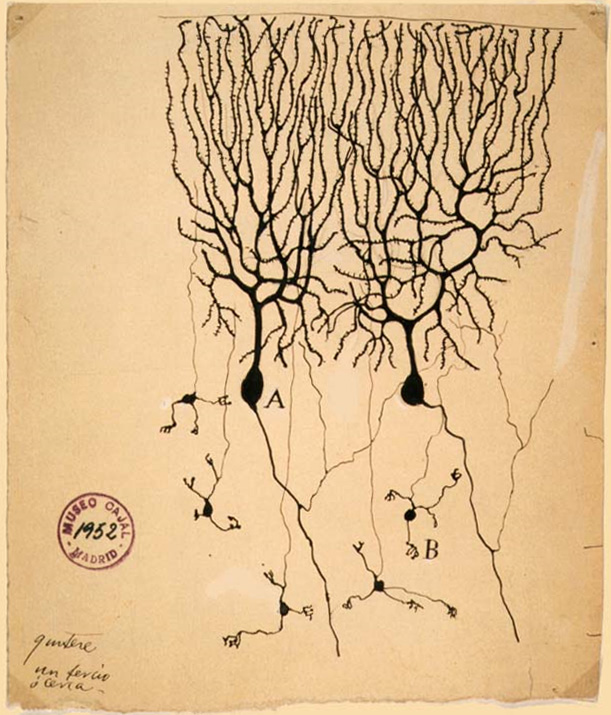
\includegraphics[width=0.30\linewidth]{images/book5/cajal-purkinje.jpg}\hspace{0.04\linewidth}
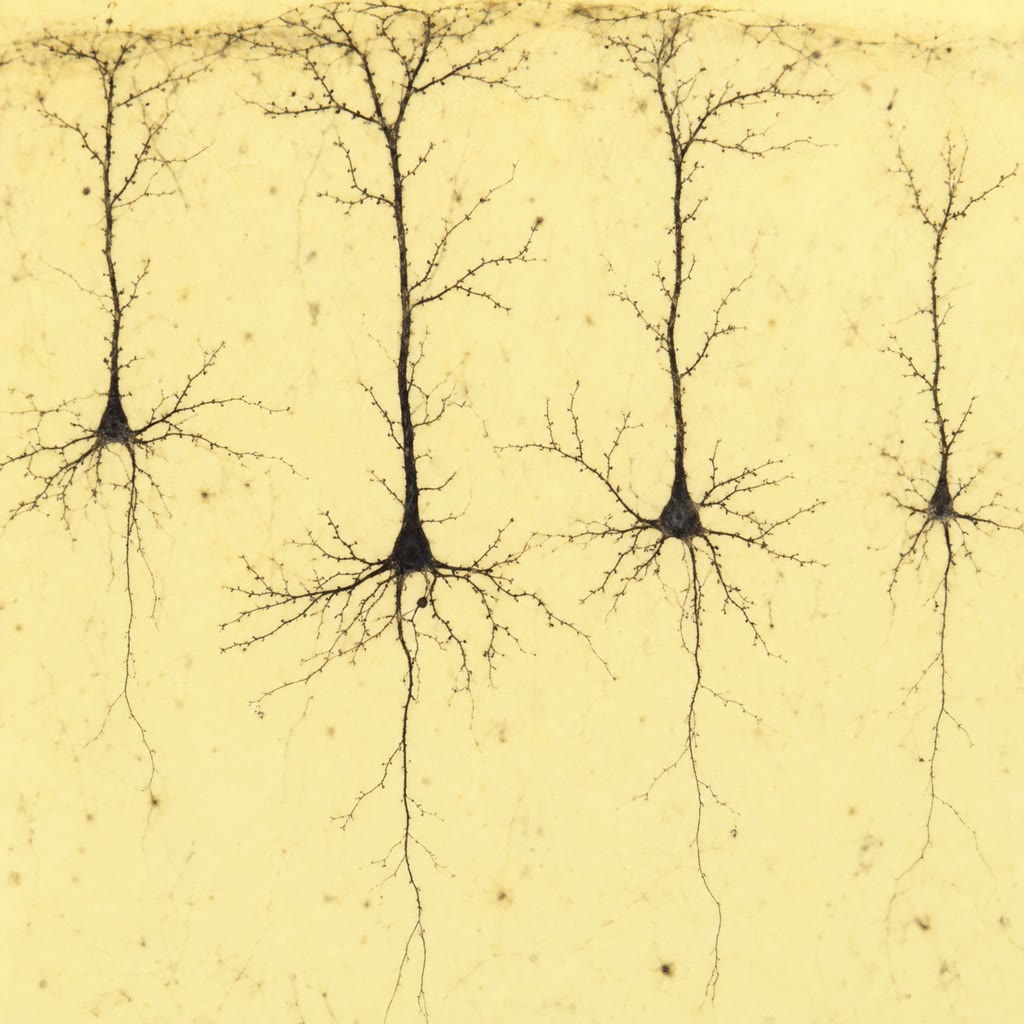
\includegraphics[width=0.30\linewidth]{images/book5/ai/b5-17-cortex-neurons.jpg}\hspace{0.04\linewidth}
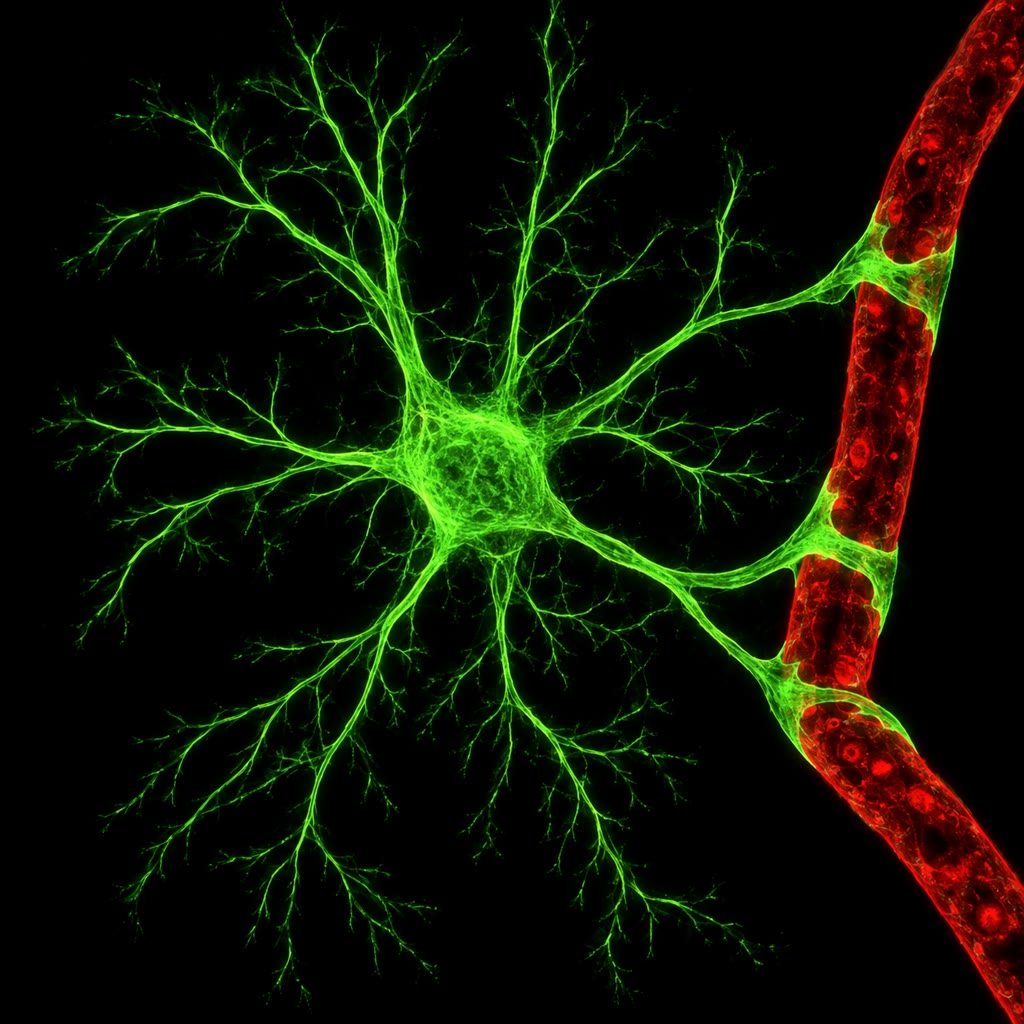
\includegraphics[width=0.30\linewidth]{images/book5/ai/b5-17-astrocyte.jpg}

{\small बाएँ: काहाल (1899) द्वारा किसी गॉल्जी-रँगी काट से बनाया गया
\omterm{def:b3:nervous-systems:plan}{अनुमस्तिष्क} की कोई पुरकिंजे कोशिका का चित्र --- किसी एक कोशिका का पूरा
द्रुमिका वृक्ष, यानी न्यूरॉन के इकाई होने का तर्क (सार्वजनिक)। बीच में:
गॉल्जी रंजन में प्रांतस्था के पिरामिडी न्यूरॉन। दाएँ: किसी केशिका (लाल)
पर अपने पादांत टिकाए कोई \omterm{def:b3:nervous-systems:cells}{तारा-कोशिका} (हरी)।}
\end{omfigure}

\section{केबल के रूप में न्यूरॉन}

\begin{theorem}[स्थायी-अवस्था केबल समीकरण]\label{thm:b3:nervous-systems:cable}
\index{केबल समीकरण}\index{लंबाई-अचर}\index{काल-अचर!झिल्ली}\index{चालन वेग}
किसी द्रुमिका या अमायलिनी तंत्रिकाक्ष को व्यास $d$ के ऐसे बेलन का
प्रतिरूप दीजिए जिसके कोशिकाद्रव्य की प्रतिरोधकता $R_{i}$ हो और जिसकी
झिल्ली का विशिष्ट प्रतिरोध $R_{m}$ (प्रतिरोध गुणा क्षेत्रफल) तथा प्रति
क्षेत्रफल धारिता $C_{m}$ हो। प्रति एकांक लंबाई अक्षीय प्रतिरोध
$r_{i} = 4R_{i}/\pi d^{2}$ है और झिल्ली-प्रतिरोध $r_{m} = R_{m}/\pi d$।
कोई स्थायी वोल्टता $V_{0}$, जो $x = 0$ पर लगाई जाए, उस तंतु पर ऐसे फैलती है
\[
V(x) = V_{0}\,e^{-x/\lambda}, \qquad
\lambda = \sqrt{\frac{r_{m}}{r_{i}}} = \sqrt{\frac{R_{m}\,d}{4R_{i}}},
\]
जहाँ $\lambda$ \emph{लंबाई-अचर} है: वह दूरी जिस पर कोई निष्क्रिय संकेत
गिरकर $1/e$ रह जाता है, और जो व्यास के वर्गमूल के साथ बढ़ती है। झिल्ली
\emph{काल-अचर} $\tau =
R_{m}C_{m}$ के साथ आवेशित होती है, जो ज्यामिति से स्वतंत्र है। कोई
क्रिया विभव, जो स्वयं को फिर-फिर जनता है, किसी अमायलिनी तंत्रिकाक्ष पर
$\lambda/\tau$ के और इसलिए $\sqrt{d}$ के समानुपाती चाल से चलता है; किसी
मायलिनी तंत्रिकाक्ष पर, जहाँ वह गाँठ से गाँठ कूदता है, $d$ के
समानुपाती चाल से --- यानी व्यास के प्रति माइक्रोमीटर लगभग
\qty{6}{m/s}।
\end{theorem}
\begin{proof}
मान लीजिए $I(x)$ अक्षीय धारा है। क्रोड के अनुदिश ओम का नियम
$\mathrm{d}V/\mathrm{d}x = -r_{i}I$ देता है; स्थायी अवस्था पर आवेश का
संरक्षण कहता है कि $x$ और $x + \mathrm{d}x$ के बीच खोई अक्षीय धारा
झिल्ली से रिस जाती है, $\mathrm{d}I/\mathrm{d}x = -V/r_{m}$। पहले का
अवकलन करके दूसरा रखने पर
$\mathrm{d}^{2}V/\mathrm{d}x^{2} = (r_{i}/r_{m})V = V/\lambda^{2}$, यानी
कोई रैखिक द्वितीय-कोटि समीकरण, जिसका $x \to \infty$ पर परिबद्ध हल
$V_{0}e^{-x/\lambda}$ है। $r_{m} = R_{m}/\pi d$ और $r_{i} =
4R_{i}/\pi d^{2}$ रखने पर $\lambda^{2} = R_{m}d/4R_{i}$ मिलता है।
काल-अचर समांतर में जुड़े किसी प्रतिरोधक और संधारित्र का है, $r_{m}c_{m} =
(R_{m}/\pi d)(C_{m}\pi d) = R_{m}C_{m}$। वेगों के लिए: फिर-फिर जनती कोई
तरंग को लगभग एक काल-अचर में एक लंबाई-अचर आगे तक झिल्ली आवेशित करनी
पड़ती है, इसलिए $v \sim \lambda/\tau \propto \sqrt{d}$; किसी मायलिनी
तंत्रिकाक्ष की गाँठों के बीच अंतरगाँठी झिल्ली का प्रतिरोध \omterm{def:b3:nervous-systems:cells}{मायलिन} के सौ
से अधिक स्तरों से बढ़ा और धारिता घटी होती है, अंतरगाँठ की लंबाई $d$ के
साथ बढ़ती है, और परिणाम $v \propto d$ है। समानुपात-अचर स्वीकार कर लिए
गए हैं।
\end{proof}

\begin{example}[किसी द्रुमिका और दो तंत्रिकाक्षों के आँकड़े]\label{ex:b3:nervous-systems:numbers}
$d = \qty{2}{\micro m}$ की कोई द्रुमिका, जिसका $R_{m} = \qty{2e4}{\ohm.cm^2}$
और $R_{i} = \qty{100}{\ohm.cm}$ हो: $\lambda = \sqrt{2\times 10^{4}\times
2\times 10^{-4}/400}\ \unit{cm} = \qty{0.1}{cm} = \qty{1}{mm}$ --- यानी
मिलीमीटर भर लंबी किसी द्रुमिका के सिरे पर उठा कोई संधि-विभव कोशिका-काया
तक अपने तिहाई आकार में पहुँचता है, और इसीलिए किसी द्रुमिका वृक्ष की
ज्यामिति उसकी संगणना का हिस्सा है। $\tau = 2\times 10^{4}\times
10^{-6}\,\unit{F/cm^2}\cdot\unit{\ohm.cm^2} = \qty{20}{ms}$, यानी वह
खिड़की जिसके भीतर निवेशों को जुड़ने के लिए पहुँचना पड़ता है।
\qty{500}{\micro m} का कोई अमायलिनी स्क्विड महा-तंत्रिकाक्ष लगभग
\qty{25}{m/s} पर चालन करता है; वही करने के लिए कोई कशेरुकी
\qty{4}{\micro m} का मायलिनी तंत्रिकाक्ष काम में लेता है, जिसकी
अनुप्रस्थ काट पंद्रह हज़ार गुना छोटी है --- यही कारण है कि कोई कशेरुकी
तंत्रिका एक स्क्विड तंत्रिकाक्ष की जगह में दस हज़ार तेज़ तंतु ढो सकती
है। \qty{20}{\micro m} का कोई प्रेरक तंत्रिकाक्ष \qty{120}{m/s} पर
चालन करता है; जब बहुखंडी काठिन्य उसका \omterm{def:b3:nervous-systems:cells}{मायलिन} उतार देता है तब वेग दस
गुना गिर जाता है और नंगे हिस्सों पर चालन पूरी तरह विफल भी हो सकता है।
\end{example}

\begin{omfigure}
\begin{tikzpicture}
\begin{axis}[
  width=6.4cm, height=5.2cm,
  axis x line=bottom, axis y line=left,
  xmin=0, xmax=3, ymin=0, ymax=1.05,
  xlabel={दूरी (mm)}, ylabel={$V/V_{0}$},
  xlabel style={font=\small, at={(axis description cs:0.5,-0.12)}, anchor=north}, ylabel style={font=\small},
  tick label style={font=\scriptsize}, xtick={0,1,2,3}, ytick={0,0.37,1}, yticklabels={0,$1/e$,1},
  clip=false,
]
\addplot[very thick, omDef, domain=0:3, samples=60] {exp(-x/1.0)};
\addplot[very thick, omThm, domain=0:3, samples=60] {exp(-x/0.5)};
\node[font=\scriptsize, omDef, anchor=south west] at (axis cs:1.2,0.45) {$d = \qty{2}{\micro m}$, $\lambda = \qty{1}{mm}$};
\node[font=\scriptsize, omThm, anchor=north west] at (axis cs:0.8,0.22) {$d = \qty{0.5}{\micro m}$, $\lambda = \qty{0.5}{mm}$};
\end{axis}
\begin{axis}[
  at={(7.6cm,0)}, anchor=south west,
  width=6.4cm, height=5.2cm,
  xmode=log, ymode=log,
  xmin=0.1, xmax=1000, ymin=0.1, ymax=200,
  xlabel={तंत्रिकाक्ष का व्यास ($\unit{\micro m}$)}, ylabel={वेग (m/s)},
  xlabel style={font=\small, at={(axis description cs:0.5,-0.12)}, anchor=north}, ylabel style={font=\small},
  tick label style={font=\scriptsize},
  clip=false,
]
\addplot[very thick, omDef, domain=1:25, samples=2] {6*x};
\addplot[very thick, omThm, domain=0.2:1000, samples=2] {1.1*sqrt(x)};
\fill[omThm] (axis cs:500,25) circle (2pt); \node[font=\scriptsize, anchor=north east] at (axis cs:500,23) {स्क्विड महा-तंत्रिकाक्ष};
\fill[omDef] (axis cs:20,120) circle (2pt); \node[font=\scriptsize, anchor=west] at (axis cs:26,120) {मानव प्रेरक तंत्रिकाक्ष};
\node[font=\scriptsize, omDef, anchor=north west, align=left] at (axis cs:1.2,60) {मायलिनी: $v \propto d$};
\node[font=\scriptsize, omThm, anchor=north west, align=left] at (axis cs:2,0.7) {अमायलिनी: $v \propto \sqrt{d}$};
\end{axis}
\end{tikzpicture}

{\small बाएँ: दो व्यासों के लिए किसी द्रुमिका पर किसी स्थायी संकेत का
निष्क्रिय क्षय --- लंबाई-अचर $\sqrt{d}$ की तरह बढ़ता है। दाएँ: व्यास के
सामने \omterm{thm:b3:nervous-systems:cable}{चालन वेग}; \omterm{def:b3:nervous-systems:cells}{मायलिन} किसी \qty{4}{\micro m} तंतु से वह करा देता है
जिसके लिए किसी अमायलिनी तंत्रिकाक्ष को आधा मिलीमीटर चाहिए।}
\end{omfigure}

\section{परिपथ}

\begin{definition}[प्राथमिक परिपथ]\label{def:b3:nervous-systems:circuits}
\index{प्रतिवर्त चाप}\index{पारस्परिक निरोध}\index{अग्रप्रवाही निरोध}\index{पुनर्भरण निरोध}\index{अभिसरण}\index{अपसरण}
कोई \emph{प्रतिवर्त चाप} किसी संवेदक से किसी कारक तक का सबसे छोटा
रास्ता है: घुटने के झटके में कोई पेशी-तर्कु अभिवाही \omterm{def:b3:nervous-systems:plan}{मेरुरज्जु} में
घुसता है और सीधे उसी पेशी के प्रेरक न्यूरॉनों पर संधि बनाता है, जो उसे
ठोकर के लगभग \qty{30}{ms} बाद सिकोड़ देते हैं --- एक संधि, कोई
मस्तिष्क नहीं। वही अभिवाही विरोधी पेशी के प्रेरक न्यूरॉनों तक जाते किसी
निरोधी \omterm{def:b3:nervous-systems:cells}{अंतर्न्यूरॉन} को उत्तेजित करता है (\emph{पारस्परिक निरोध}), ताकि
प्रसारक का संकुचन आकुंचक से न लड़े। अधिकांश परिपथ कुछ ही नमूनों से बने
हैं: \emph{अपसरण}, यानी एक न्यूरॉन का अनेक को चलाना, और
\emph{अभिसरण}, यानी अनेक का एक पर, जो साक्ष्य जोड़ता है;
\emph{अग्रप्रवाही निरोध}, जिसमें कोई निवेश किसी लक्ष्य को और किसी ऐसे
\omterm{def:b3:nervous-systems:cells}{अंतर्न्यूरॉन} को भी उत्तेजित करता है जो मिलीसेकंड भर बाद उस लक्ष्य का
निरोध कर देता है, जिससे अनुक्रिया समय में तीखी होती है; \emph{पुनर्भरण
निरोध}, जिसमें लक्ष्य का अपना निर्गम किसी ऐसे \omterm{def:b3:nervous-systems:cells}{अंतर्न्यूरॉन} को उत्तेजित
करता है जो उसी का निरोध करता है, जिससे दगना सीमित होता है और, पड़ोसियों
तक फैलकर, वह पार्श्व निरोध पैदा होता है जो विपर्यास तीखा करता है
(\cref{ch:b3:sensory-systems}); और \emph{निरोध-मोचन}, यानी किसी निरोधक
का निरोध, जो आधारीय \omterm{def:b3:nervous-systems:comparative}{गंडिकाओं} का कोई गति छोड़ने का ढंग है।
\end{definition}

\begin{omfigure}
\begin{tikzpicture}[every node/.style={font=\scriptsize}, >=stealth]
  % spinal cord cross-section (schematic)
  \draw[thick, omDef!60, fill=omDef!8] (5.4,1.5) ellipse (2.0 and 1.5);
  \draw[thick, gray, fill=gray!15] (5.4,1.5) .. controls (4.7,2.4) and (4.0,2.6) .. (4.0,1.9) .. controls (4.0,1.2) and (4.6,0.9) .. (4.8,0.5) .. controls (5.0,0.2) and (5.8,0.2) .. (6.0,0.5) .. controls (6.2,0.9) and (6.8,1.2) .. (6.8,1.9) .. controls (6.8,2.6) and (6.1,2.4) .. (5.4,1.5);
  \node[above] at (5.4,3.05) {मेरुरज्जु};
  % muscles
  \draw[thick, omMeth!70!black, fill=omMeth!20] (0.2,0.2) rectangle (1.4,2.0); \node[below, align=center] at (0.8,0.1) {प्रसारक\\(चतुःशिरस्क)};
  \draw[thick, omThm!70!black, fill=omThm!15] (0.2,-2.6) rectangle (1.4,-1.4); \node[below, align=center] at (0.8,-2.7) {आकुंचक\\(पश्चजंघ)};
  \fill[omProp] (0.8,1.3) ellipse (0.12 and 0.3); \node[left, font=\tiny] at (0.65,1.3) {तर्कु};
  % Ia afferent to cord (dorsal)
  \draw[very thick, omProp] (0.9,1.3) .. controls (2.0,2.6) and (3.6,2.9) .. (4.8,2.2); \fill[omProp] (4.8,2.2) circle (0.09);
  \node[above, omProp] at (2.6,2.85) {Ia अभिवाही: तनाव};
  % motor neuron to extensor
  \fill[omMeth!70!black] (5.0,0.9) circle (0.16);
  \draw[->, very thick, omMeth!70!black] (4.9,0.85) .. controls (3.4,0.3) and (2.0,0.4) .. (1.4,1.0);
  \draw[->, thick, omProp] (4.8,2.2) -- (5.0,1.1);
  % inhibitory interneuron to flexor motor neuron
  \fill[omThm] (6.1,1.7) circle (0.13);
  \draw[->, thick, omProp] (4.9,2.25) -- (6.0,1.8);
  \fill[omThm!70!black] (6.0,0.6) circle (0.16);
  \draw[-|, thick, omThm] (6.1,1.55) -- (6.0,0.8);
  \draw[->, very thick, omThm!70!black, dashed] (5.9,0.5) .. controls (4.8,-0.8) and (3.0,-1.6) .. (1.4,-2.0);
  % right-hand labels with leaders
  \node[right, omThm, font=\tiny] at (7.6,1.9) {Ia निरोधी अंतर्न्यूरॉन}; \draw[gray, thin] (7.55,1.9) -- (6.25,1.7);
  \node[right, omMeth!70!black, font=\tiny, align=left] at (7.6,1.1) {प्रसारक का प्रेरक न्यूरॉन: उत्तेजित}; \draw[gray, thin] (7.55,1.1) -- (5.15,0.9);
  \node[right, omThm!70!black, font=\tiny, align=left] at (7.6,0.3) {आकुंचक का प्रेरक न्यूरॉन: निरोधित}; \draw[gray, thin] (7.55,0.3) -- (6.15,0.6);
  \node[below] at (4.6,-0.15) {एकसंधिक प्रतिवर्त: $\sim$\qty{30}{ms}};
  \node[below, align=center] at (4.2,-2.0) {पारस्परिक निरोध:\\प्रतिपक्षी ढीला पड़ता है};
\end{tikzpicture}

{\small तनाव-प्रतिवर्त। कोई ठोकर प्रसारक के तर्कु खींचती है; Ia अभिवाही
प्रसारक के प्रेरक न्यूरॉनों को सीधे (एक संधि से) उत्तेजित करता है और,
किसी निरोधी \omterm{def:b3:nervous-systems:cells}{अंतर्न्यूरॉन} के ज़रिए, आकुंचक के न्यूरॉन चुप करा देता है।}
\end{omfigure}

\begin{proposition}[केंद्रीय प्ररूप-जनित्र]\label{prop:b3:nervous-systems:cpg}
\index{केंद्रीय प्ररूप-जनित्र}\index{अर्ध-केंद्र दोलक}
लयबद्ध गतियाँ --- साँस लेना, चलना, तैरना, चबाना --- \omterm{def:b3:nervous-systems:plan}{मस्तिष्क-स्तंभ} और
\omterm{def:b3:nervous-systems:plan}{मेरुरज्जु} के उन परिपथों से बनती हैं जो अपने आप दोलन करते हैं, यानी
\emph{\omterm{prop:b3:nervous-systems:cpg}{केंद्रीय प्ररूप-जनित्र}}, जिन्हें संवेदी पुनर्भरण समायोजित करता है,
बनाता नहीं: किसी बिल्ली की \omterm{def:b3:nervous-systems:plan}{मेरुरज्जु} मस्तिष्क से काट दी जाए और उसकी
संवेदी तंत्रिकाएँ भी हटा दी जाएँ, फिर भी वह कदम बढ़ाने का एकांतर प्ररूप
बनाती है। सबसे सरल अभिकल्प ब्राउन का \emph{अर्ध-केंद्र} (1911) है:
न्यूरॉनों के दो समूह, जिनमें हर एक दूसरे का निरोध करता है। जो भी दगे वह
अपने साथी को चुप करा देता है; पर दगता समूह थक जाता है --- उसकी
वाहिकाएँ निष्क्रियित होती हैं, साथी पर उसका निरोध कमज़ोर पड़ता है ---
और छूट पाकर साथी दगता है और बदले में पहले को चुप करा देता है: यानी
एकांतरण, जिसका आवर्तकाल किसी घड़ी से नहीं, उस थकान के काल-अचर से तय
होता है। श्वसन-लय मेडुला के कुछ हज़ार न्यूरॉनों के किसी गुच्छे (पूर्व
बॉट्ज़िंगर संकुल) में उठती है, जो जन्म से मृत्यु तक झोंकों में दगता है;
लैंप्रे का तैरना उसकी रज्जु के अनुदिश अर्ध-केंद्रों की कोई शृंखला है,
जिनमें हर एक पिछले से पिछड़ा हुआ है ताकि कोई तरंग पूँछ की ओर चले।
\end{proposition}

\begin{omfigure}
\begin{tikzpicture}[every node/.style={font=\scriptsize}, >=stealth]
  % half-centre
  \begin{scope}
    \draw[thick, fill=omDef!25] (0,0) circle (0.5); \node at (0,0) {बा};
    \draw[thick, fill=omThm!25] (3,0) circle (0.5); \node at (3,0) {दा};
    \draw[-|, very thick] (0.5,0.2) -- (2.5,0.2); \draw[-|, very thick] (2.5,-0.2) -- (0.5,-0.2);
    \node[above] at (1.5,0.3) {पारस्परिक निरोध};
    \draw[->, thick, omDef] (0,-0.5) -- (0,-1.3) node[below] {बाईं पेशियाँ};
    \draw[->, thick, omThm] (3,-0.5) -- (3,-1.3) node[below] {दाईं पेशियाँ};
    \draw[->, thick, gray] (-1.2,0.6) -- (-0.45,0.25) node[pos=0, above, align=center] {मस्तिष्क-स्तंभ से\\अविरत चालन};
    \draw[->, thick, gray] (4.5,0.6) -- (3.45,0.25);
  \end{scope}
  % traces
  \begin{scope}[xshift=6.0cm, yshift=0.9cm]
    \node[left, omDef] at (0,0) {बा};
    \foreach \x in {0,2,4} { \foreach \s in {0.1,0.2,...,0.9} \draw[omDef] (\x+\s,-0.15) -- (\x+\s,0.15); }
    \node[left, omThm] at (0,-1.0) {दा};
    \foreach \x in {1,3,5} { \foreach \s in {0.1,0.2,...,0.9} \draw[omThm] (\x+\s,-1.15) -- (\x+\s,-0.85); }
    \draw[->] (0,-1.6) -- (6.2,-1.6) node[right] {समय};
    \draw[<->] (0,-2.0) -- (2,-2.0) node[midway, below] {आवर्तकाल: थकान से तय};
  \end{scope}
\end{tikzpicture}

{\small कोई \omterm{prop:b3:nervous-systems:cpg}{अर्ध-केंद्र दोलक}। स्थिर चालन के अंतर्गत दो परस्पर निरोधी
समूह एकांतर करते हैं: सक्रिय पक्ष थकता है, उसका निरोध कमज़ोर पड़ता है,
दूसरा पक्ष छूटकर बागडोर सँभाल लेता है। कोई भी न्यूरॉन स्वयं लयबद्ध
नहीं है।}
\end{omfigure}

\begin{method}[किसी परिपथ का अनुरेखण]\label{met:b3:nervous-systems:tracing}
\index{परिपथ-अनुरेखण}\index{प्रकाश-आनुवंशिकी}
यह स्थापित करने के लिए कि न्यूरॉन A न्यूरॉन B को चलाता है और वह पथ किसी
व्यवहार के लिए मायने रखता है: (1) शारीरिकी --- कोई ऐसा अनुरेखक
अंतःक्षिप्त कीजिए जो तंत्रिकाक्षों के अनुदिश चलता हो (कोई रंजक, कोई
रूपांतरित रेबीज़ \omterm{def:b3:virology:virus}{विषाणु} जो एक संधि पीछे की ओर पार करता है) और जुड़ी हुई
कोशिकाएँ खोजिए; (2) शरीरक्रिया --- A को उद्दीपित करते हुए B से अभिलेख
लीजिए, और विलंब (कोई एकसंधिक संयोजन लगभग मिलीसेकंड भर का नियत विलंब
देता है) तथा चिह्न (उत्तेजन या निरोध) नापिए; (3) आवश्यकता --- A को
चुप कीजिए, किसी क्षति से, ठंडा करके, या उसमें कोई प्रकाश-चालित
क्लोराइड पंप अभिव्यक्त करके और प्रकाश डालकर (\emph{प्रकाश-आनुवंशिकी}),
और देखिए कि क्या वह व्यवहार विफल होता है; (4) पर्याप्तता --- किसी
प्रकाश-चालित धनायन वाहिका से अकेले A को सक्रिय कीजिए और देखिए कि क्या
वह व्यवहार प्रकट होता है; (5) किसी अक्षत प्राणी में, व्यवहार होते समय
किसी कैल्सियम सूचक से पूरी समष्टि की क्रियाशीलता का प्रतिबिंबन कीजिए।
कोई परिपथ तब स्थापित होता है जब पाँचों सहमत हों; अधिकांश प्रकाशित
परिपथों के पास दो या तीन हैं।
\end{method}

\section{कशेरुकी तंत्रिका-तंत्र की योजना}

\begin{definition}[केंद्रीय और परिधीय भाग]\label{def:b3:nervous-systems:plan}
\index{मेरुरज्जु}\index{मस्तिष्क-स्तंभ}\index{अनुमस्तिष्क}\index{चेतक}\index{अधश्चेतक}\index{प्रमस्तिष्क प्रांतस्था}\index{स्वायत्त तंत्रिका-तंत्र}\index{आंत्रिक तंत्रिका-तंत्र}
\emph{केंद्रीय तंत्रिका-तंत्र} मस्तिष्क और मेरुरज्जु है;
\emph{परिधीय} बाकी सब कुछ। \emph{मेरुरज्जु} अपने पृष्ठीय मूलों से संवेदी
तंत्रिकाक्ष लेती है और अपने अधर मूलों से प्रेरक तंत्रिकाक्ष भेजती है;
उसका धूसर पदार्थ कोशिका-कायाओं की कोई तितली है और उसका श्वेत पदार्थ
ऊपर-नीचे दौड़ते मायलिनी पथ। \emph{मस्तिष्क-स्तंभ} --- मेडुला, पोंस,
मध्यमस्तिष्क --- कपाल तंत्रिकाओं की गुठलियाँ और वे केंद्र रखता है जो
बिना सोचे साँस, हृद्-दर और रक्तचाप चलाए रखते हैं; मस्तिष्क-स्तंभ की
मृत्यु मृत्यु है। \emph{अनुमस्तिष्क}, जिसमें बाकी मस्तिष्क से अधिक
न्यूरॉन हैं, गति के समय-निर्धारण और समन्वय को सुर में करता है और त्रुटि
से सीखता है। \emph{चेतक} गंध को छोड़ हर संवेदन को प्रांतस्था तक और
प्रांतस्था के उत्तर वापस पहुँचाता है; उसके नीचे बैठा \emph{अधश्चेतक}
समस्थापन चलाता है --- तापमान, भूख, प्यास, घड़ी,
\cref{ch:b3:endocrinology} के अंतःस्रावी अक्ष। \emph{आधारीय
\omterm{def:b3:nervous-systems:comparative}{गंडिकाएँ}} संभव क्रियाओं में से चुनती हैं; \emph{हिप्पोकैम्पस} स्मृतियाँ
बनाता है (\cref{ch:b3:learning-memory}); और \emph{प्रमस्तिष्क
प्रांतस्था}, यानी कोशिकाओं की छह परतों की कोई दो से चार मिलीमीटर मोटी
और चौथाई वर्ग मीटर क्षेत्रफल की चादर, जो समाने के लिए मोड़ी गई है,
बाकी सब करती है, हर संवेदन तथा गति के लिए मानचित्रित क्षेत्रों में और
उनके बीच पड़े साहचर्य क्षेत्रों में। परिधीय तंत्र का \emph{स्वायत्त}
भाग अंग चलाता है: \emph{अनुकंपी} शृंखला, जो नॉरएड्रिनैलीन छोड़कर
लामबंद करती है (हृदय ऊपर, आँत नीचे, पुतलियाँ चौड़ी);
\emph{परानुकंपी} तंत्रिकाएँ, जो ऐसीटिलकोलीन छोड़कर बचाती और पचाती हैं;
और \emph{आंत्रिक} तंत्रिका-तंत्र, यानी आँत की दीवार में बैठे आधा अरब
न्यूरॉन, जो पाचन अपने आप चलाते हैं।
\end{definition}

\begin{omfigure}
\begin{tikzpicture}[every node/.style={font=\scriptsize}, >=stealth]
  % sagittal brain schematic
  \draw[thick, omDef!70, fill=omDef!15] (0,2.0) .. controls (0,4.6) and (3.5,5.4) .. (6.0,4.4) .. controls (7.6,3.7) and (7.4,2.2) .. (6.2,1.9) .. controls (5.4,1.7) and (5.2,1.3) .. (4.4,1.6) .. controls (3.0,1.3) and (1.2,1.4) .. (0,2.0);
  \node[align=center] at (3.0,3.9) {प्रमस्तिष्क प्रांतस्था: छह परतें,\\संवेदी, प्रेरक और साहचर्य क्षेत्र};
  % basal ganglia / hippocampus (deep)
  \draw[thick, omProp!70, fill=omProp!25] (3.2,2.6) ellipse (0.9 and 0.45); \node[font=\tiny] at (3.2,2.6) {आधारीय गंडिकाएँ};
  \draw[thick, omProp!70, fill=omProp!25] (5.2,2.45) ellipse (0.88 and 0.3); \node[font=\tiny] at (5.2,2.45) {हिप्पोकैम्पस};
  % thalamus, hypothalamus
  \draw[thick, omMeth!70!black, fill=omMeth!25] (4.0,1.95) ellipse (0.7 and 0.3); \node[font=\tiny] at (4.0,1.95) {चेतक};
  \draw[thick, omMeth!70!black, fill=omMeth!40] (4.0,1.42) ellipse (0.78 and 0.22); \node[font=\tiny] at (4.0,1.42) {अधश्चेतक};
  % cerebellum
  \draw[thick, omThm!70, fill=omThm!20] (6.6,1.2) ellipse (0.9 and 0.6); \node[font=\tiny] at (6.6,1.2) {अनुमस्तिष्क};
  % brainstem
  \draw[thick, gray!70, fill=gray!20] (4.7,1.2) -- (5.5,1.2) -- (5.9,-0.3) -- (5.1,-0.3) -- cycle; \node[font=\tiny, rotate=-75] at (5.3,0.45) {मस्तिष्क-स्तंभ};
  % spinal cord
  \draw[thick, gray!70, fill=gray!20] (5.2,-0.3) rectangle (5.8,-1.6); \node[right, font=\tiny] at (5.85,-1.0) {मेरुरज्जु};
  % labels with leaders on the right
  \node[right, align=left] at (7.8,3.4) {चेतक: गंध को छोड़ हर संवेदन\\का प्रसारक; अधश्चेतक:\\समस्थापन, घड़ी, अंतःस्रावी अक्ष};
  \draw[gray] (7.75,3.3) -- (4.7,1.95);
  \node[right, align=left] at (7.8,1.9) {अनुमस्तिष्क: समय-निर्धारण और\\समन्वय, त्रुटि से सीखना};
  \draw[gray] (7.75,1.8) -- (7.5,1.4);
  \node[right, align=left] at (7.8,0.4) {मस्तिष्क-स्तंभ: साँस, हृदय,\\कपाल तंत्रिकाएँ (मेडुला,\\पोंस, मध्यमस्तिष्क)};
  \draw[gray] (7.75,0.4) -- (5.9,0.4);
  \node[right, align=left] at (7.8,-1.0) {मेरुरज्जु: प्रतिवर्त, प्ररूप-जनित्र,\\ऊपर-नीचे जाते पथ};
\end{tikzpicture}

{\small कशेरुकी मस्तिष्क का धनु दृश्य, योजनाबद्ध: गहरी गुठलियों के ऊपर
प्रांतस्था, केंद्र में \omterm{def:b3:nervous-systems:plan}{चेतक} तथा \omterm{def:b3:nervous-systems:plan}{अधश्चेतक}, पीछे \omterm{def:b3:nervous-systems:plan}{अनुमस्तिष्क}, और
\omterm{def:b3:nervous-systems:plan}{मस्तिष्क-स्तंभ}, जो \omterm{def:b3:nervous-systems:plan}{मेरुरज्जु} में जाकर मिलता है।}
\end{omfigure}

\begin{proposition}[रक्त--मस्तिष्क अवरोध और मस्तिष्क का बजट]\label{prop:b3:nervous-systems:barrier-budget}
\index{रक्त-मस्तिष्क अवरोध}\index{प्रमस्तिष्क-मेरु द्रव}\index{मस्तिष्क का ऊर्जा-बजट}
मस्तिष्क की केशिकाएँ अपनी अंतःस्तरी कोशिकाओं के बीच के दृढ़ जोड़ों से
सील हैं, \omterm{def:b3:nervous-systems:cells}{तारा-कोशिकाओं} के पादांतों में लिपटी हैं, और ऐसे वाहकों से
सज्जित जो ग्लूकोस तथा ऐमीनो अम्ल भीतर आने देते हैं और बहुत कुछ बाहर
पंप कर देते हैं: यही \emph{रक्त--मस्तिष्क अवरोध} है, जो न्यूरॉनों के
वैद्युत व्यवहार की ख़ातिर मस्तिष्क के बाह्यकोशिकीय द्रव का आयनी संघटन
अचर रखता है, और जो अधिकांश औषधें बाहर रखता है (छोटे अणुओं का
\qty{98}{\%}, सारे \omterm{def:b3:adaptive-immunity:antibody}{प्रतिरक्षी}) --- यही तंत्रिका-औषध-विज्ञान की केंद्रीय
समस्या है। मस्तिष्क \qty{150}{mL} \emph{\omterm{prop:b3:nervous-systems:barrier-budget}{प्रमस्तिष्क-मेरु द्रव}} में
तैरता है, जो मिनट भर में आधा मिलीलीटर बनता है और दिन में चार बार नया हो
जाता है, जो उसे गद्दी देता है और कचरा बहा ले जाता है, ख़ासकर नींद में।
मस्तिष्क की लागत: किसी वयस्क में कोई \qty{20}{W}, यानी विश्रामी उपापचय
का \qty{20}{\%}, लगभग सारा ATP के लिए जलाए गए ग्लूकोस के रूप में, और
उसमें से अधिकांश ATP सोडियम पंप उन प्रवणताओं को लौटाने में खर्च करता है
जिन्हें क्रिया विभव तथा संधि-धाराएँ चुका देती हैं। प्रति मोल ATP
\qty{50}{kJ} पर, \qty{20}{W} प्रति सेकंड $4\times 10^{-4}$ मोल
ATP है, यानी $2.4\times 10^{20}$ अणु; $8.6\times 10^{10}$ न्यूरॉनों में
बाँटने पर प्रति न्यूरॉन प्रति सेकंड लगभग $3\times 10^{9}$ ATP। अपने
संधि-परिणामों समेत किसी प्रांतस्थीय क्रिया विभव की लागत $10^{9}$ ATP की
कोटि की है, इसलिए वह बजट प्रति न्यूरॉन प्रति सेकंड कुछ ही आवेगों की औसत
दगने-दर की छूट देता है --- और प्रांतस्था के न्यूरॉन लगभग उसी दर से दगते
भी हैं। मस्तिष्क किसी कड़ी ऊर्जा-सीमा पर बना है, और इसीलिए उसके संकेत
विरल हैं, उसके तंत्रिकाक्ष पतले, और उसकी सूचना अनेक कोशिकाओं में थोड़े
आवेगों से कूटबद्ध।
\end{proposition}
\admitted

\section{प्राणियों भर में तंत्रिका-तंत्र}

\begin{definition}[तंत्रिका जाल, गंडिकाएँ और मस्तिष्क]\label{def:b3:nervous-systems:comparative}
\index{तंत्रिका जाल}\index{गंडिका}\index{शीर्षीकरण}\index{मस्तिष्कीकरण}
निडारियों (जेलीमीन, हाइड्रा) के पास कोई \emph{तंत्रिका जाल} है:
देह-भित्ति भर में बँटे न्यूरॉन, हर दिशा में जुड़े, और घंटी के किनारे के
चारों ओर वलयाकार सघनन, जो तैरने का समन्वय करते हैं --- कोई केंद्र नहीं,
और हर कोशिका के अनुदिश दोनों दिशाओं में चालन। द्विपार्श्वी प्राणी
न्यूरॉनों को \emph{गंडिकाओं} में सघन करते हैं --- यानी साझा न्यूरोपिल
वाले गुच्छों में --- जो संधिपादों तथा वलयकृमियों में किसी अधर रज्जु के
अनुदिश सजे हैं, और जहाँ इंद्रियाँ हैं वहाँ कोई शीर्ष-गंडिका बड़ी हुई
है: यही \emph{शीर्षीकरण} है। मोलस्क किसी सीपी की सरल गंडिकाओं से लेकर
ऑक्टोपस तक भिन्न हैं, जिसके आधा अरब न्यूरॉन किसी भी अकशेरुकी में सबसे
अधिक हैं और जिनके दो-तिहाई भुजाओं में पड़े हैं, और हर भुजा की रज्जु
अपना ही पहुँचना तथा पकड़ना चलाती है। कशेरुकी कोई पृष्ठीय खोखली नली
बनाते हैं, जो आगे की ओर पिछले खंड के मस्तिष्क में फैली है, हड्डी तथा
किसी अवरोध से सुरक्षित, और मायलिनी। वही संकेतक अणु, वाहिकाएँ,
संचारक और वही अनेक परिवर्धनी जीन (पश्चमस्तिष्क का Hox कूट,
नेत्र-प्रतिरूपक कारक) इन सबको चलाते हैं: पुर्जे प्राचीन और साझा हैं,
सजावटें विविध।
\end{definition}

\begin{example}[न्यूरॉन गिनना]\label{ex:b3:nervous-systems:counts}
किसी सूत्रकृमि के $302$ न्यूरॉन हैं, हर एक नामांकित और हर संधि
मानचित्रित; किसी फल-मक्खी के $1.4\times 10^{5}$; किसी मधुमक्खी के
$10^{6}$; किसी चूहे के $7\times 10^{7}$; किसी ऑक्टोपस के $5\times 10^{8}$;
किसी मनुष्य के $8.6\times
10^{10}$; किसी हाथी के
$2.6\times 10^{11}$, जिनमें से अधिकांश उसके \omterm{def:b3:nervous-systems:plan}{अनुमस्तिष्क} में।
स्तनियों भर में मस्तिष्क-द्रव्यमान देह-द्रव्यमान के साथ मोटे तौर पर
$M_{\text{मस्तिष्क}} \propto M_{\text{देह}}^{0.75}$ की तरह बढ़ता है,
इसलिए किसी चूहे का मस्तिष्क उसके शरीर का किसी हाथी के मस्तिष्क से बड़ा
अंश है; जो जातियाँ अपने आकार के लिए उस रेखा से ऊपर हैं --- डॉल्फ़िन,
नरवानर, और मनुष्य सात गुने से --- वे मस्तिष्कीकृत कही जाती हैं।
संज्ञान का सबसे अच्छा पीछा मस्तिष्क-द्रव्यमान नहीं, \omterm{def:b3:nervous-systems:plan}{प्रमस्तिष्क
प्रांतस्था} के न्यूरॉनों की संख्या करती है: किसी मनुष्य में लगभग
$1.6\times 10^{10}$, तीन गुने बड़े मस्तिष्क वाले हाथी में
$5.6\times 10^{9}$, किसी चिंपैंज़ी में $2\times 10^{9}$। मानव मस्तिष्क
अपनी कोशिकाओं या अपनी योजना में कुछ ख़ास नहीं है; उसके पास किसी भी
दूसरे से अधिक प्रांतस्थीय न्यूरॉन हैं, जो अधिक सघनता से भरे हैं, और
लगता है कि गिनती ही गिनी जाती है, भार नहीं।
\end{example}

\begin{omfigure}
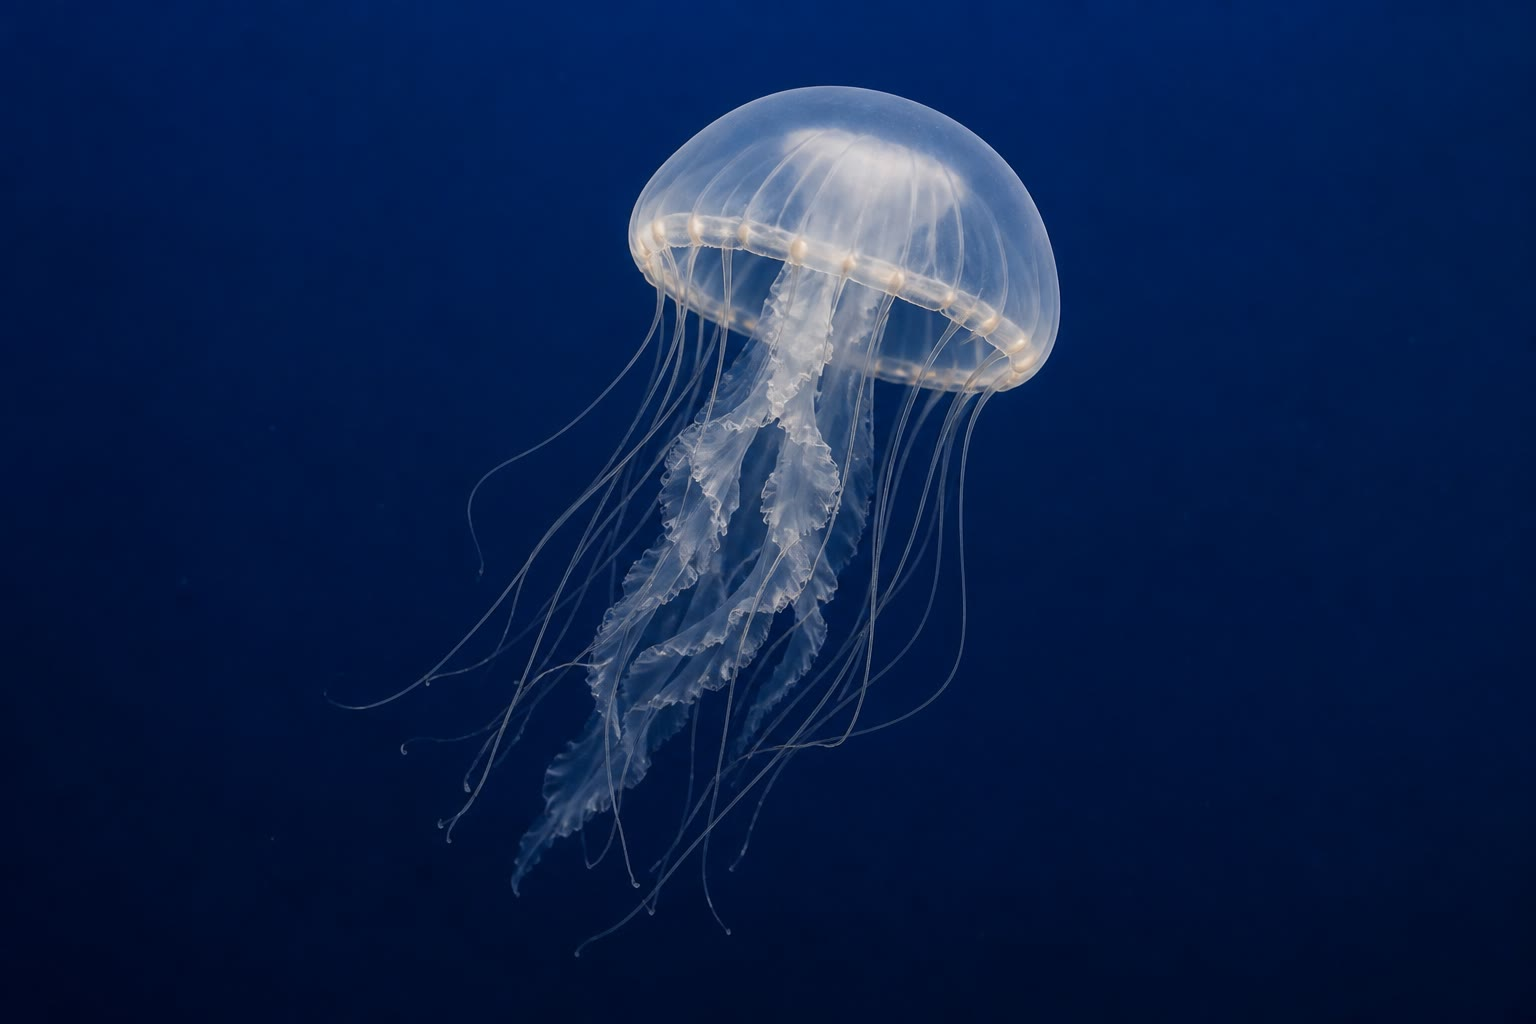
\includegraphics[width=0.46\linewidth]{images/book5/ai/b5-17-jellyfish.jpg}\hspace{0.04\linewidth}
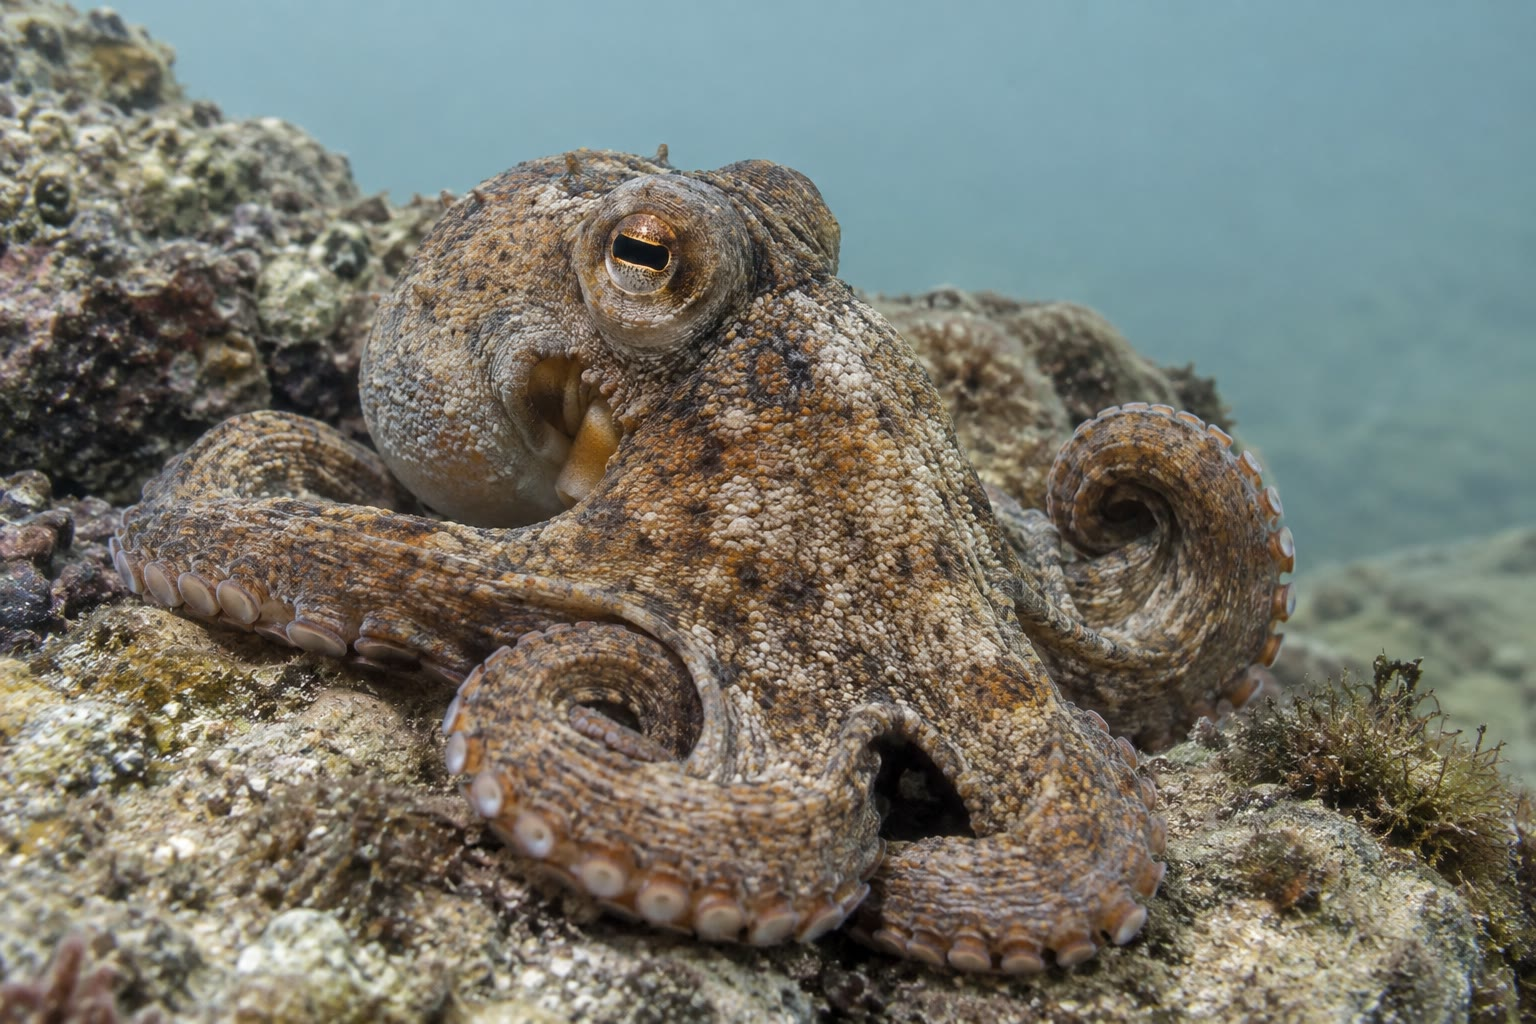
\includegraphics[width=0.46\linewidth]{images/book5/ai/b5-17-octopus.jpg}

{\small न्यूरॉन सजाने के दो ढंग। बाएँ: कोई जेलीमीन, जिसका \omterm{def:b3:nervous-systems:comparative}{तंत्रिका जाल}
और किनारे के वलय बिना किसी मस्तिष्क के तैरने का समन्वय करते हैं। दाएँ:
कोई ऑक्टोपस, जिसके आधा अरब न्यूरॉन हैं, अधिकांश भुजाओं में, और जिसका
मस्तिष्क किसी भी अकशेरुकी से बड़ा है।}
\end{omfigure}

\begin{remark}[तंत्रिका-तंत्र किस काम का है]\label{rem:b3:nervous-systems:for}
पौधों, कवकों और स्पंजों के पास कोई नहीं है; जो प्राणी चलता है उसे एक
चाहिए, और तंत्रिका-तंत्रों की विस्तृति गति की, दूर से भाँपने की, और यह
पूर्वानुमान करने की माँगों के पीछे चलती है कि आगे क्या होने वाला है।
\omterm{thm:b3:nervous-systems:cable}{केबल समीकरण} भौतिकी तय करता है --- किसी दिए व्यास और रोधन के लिए कोई
संकेत कितनी दूर और कितनी तेज़ चलता है; ऊर्जा-बजट अर्थशास्त्र तय करता
है; और उन्हीं सीमाओं के भीतर वही न्यूरॉन, जालों, \omterm{def:b3:nervous-systems:comparative}{गंडिकाओं} या किसी
प्रांतस्था के रूप में सजे हुए, किसी जेलीमीन की धड़कन, किसी ऑक्टोपस का
छद्मावरण या यह वाक्य बनाते हैं। अगले दो अध्याय निवेश-सिरा और भंडारण
उठाते हैं: इंद्रियाँ संसार को आवेगों में कैसे बदलती हैं, और
तंत्रिका-संधियाँ कैसे बदलती हैं ताकि संसार, एक बार मिल जाने पर, याद रहे।
\end{remark}

\section{अभ्यास}

\begin{exercise}[$\star$]\label{exo:b3:nervous-systems:1}
\omterm{def:b3:nervous-systems:cells}{ग्लिया} के चारों प्रकार और हर एक का एक-एक प्रकार्य बताइए, और यह भी कि
उनमें से कौन-से दो \omterm{def:b3:nervous-systems:cells}{मायलिन} बनाते हैं और कहाँ।
\end{exercise}

\begin{exercise}[$\star$]\label{exo:b3:nervous-systems:2}
गॉल्जी के रंजन ने क्या संभव किया, काहाल ने उससे क्या निष्कर्ष निकाला,
और गॉल्जी ने क्या? कौन सही था, और यह तय कैसे हुआ?
\end{exercise}

\begin{exercise}[$\star$]\label{exo:b3:nervous-systems:3}
घुटने-झटके के \omterm{def:b3:nervous-systems:circuits}{प्रतिवर्त चाप} का वर्णन कीजिए और समझाइए कि उसमें केवल
\qty{30}{ms} क्यों लगते हैं जबकि किसी ऐच्छिक लात में दस गुना अधिक।
\end{exercise}

\begin{exercise}[$\star$]\label{exo:b3:nervous-systems:4}
हृदय, पुतली, आँत और वायुमार्गों पर अनुकंपी तथा परानुकंपी प्रभाव
गिनाइए, और हर भाग लक्ष्य पर जो संचारक काम में लेता है वह भी।
\end{exercise}

\begin{exercise}[$\star\star$]\label{exo:b3:nervous-systems:5}
\qty{1}{\micro m} के किसी ऐसे तंत्रिकाक्ष का लंबाई-अचर निकालिए जिसका $R_{m}
= \qty{1e4}{\ohm.cm^2}$ और $R_{i} = \qty{100}{\ohm.cm}$ हो, और
\qty{2}{mm} के बाद बचे संकेत का अंश। कौन-सा व्यास $\lambda$ दुगुना कर
देगा?
\end{exercise}

\begin{exercise}[$\star\star$]\label{exo:b3:nervous-systems:6}
पैर की उँगली से \omterm{def:b3:nervous-systems:plan}{मेरुरज्जु} तक \qty{12}{\micro m} का कोई संवेदी
तंत्रिकाक्ष \qty{1.2}{m} चलता है, और \qty{15}{\micro m} का कोई प्रेरक
तंत्रिकाक्ष वापस। प्रति माइक्रोमीटर \qty{6}{m/s} और प्रति संधि
\qty{0.5}{ms} के साथ, एक \omterm{def:b3:nervous-systems:cells}{अंतर्न्यूरॉन} वाले किसी मेरु प्रत्याहरण
प्रतिवर्त का न्यूनतम विलंब आँकिए। उतने ही व्यास के अमायलिनी
तंत्रिकाक्षों के साथ, $v = 1.1\sqrt{d}$ पर, कितना समय लगता?
\end{exercise}

\begin{exercise}[$\star\star$]\label{exo:b3:nervous-systems:7}
\cref{prop:b3:nervous-systems:barrier-budget} के मस्तिष्क-बजट का
उपयोग करते हुए आँकिए कि कोई न्यूरॉन प्रति सेकंड कितने ATP खर्च कर सकता
है, और यदि अपनी संधियों समेत किसी आवेग की लागत
$2\times 10^{9}$ ATP हो तो वह बजट कौन-सी औसत दगने-दर की छूट देता है। यह
कूट के बारे में क्या पूर्वानुमान करता है?
\end{exercise}

\begin{exercise}[$\star\star$]\label{exo:b3:nervous-systems:8}
समझाइए कि किसी \omterm{prop:b3:nervous-systems:cpg}{अर्ध-केंद्र दोलक} को दोलन के लिए थकान (या कोई दूसरी धीमी
प्रक्रिया) क्यों चाहिए, और परस्पर निरोधी ऐसे दो न्यूरॉनों के साथ क्या
होता जो कभी न थकते।
\end{exercise}

\begin{exercise}[$\star\star$]\label{exo:b3:nervous-systems:9}
रक्त--मस्तिष्क अवरोध L-डोपा के उत्पाद डोपामीन को बाहर रखता है पर
L-डोपा को भीतर आने देता है। समझाइए कि पार्किंसन रोग में इसका दोहन कैसे
होता है और मस्तिष्क-प्रोटीनों के विरुद्ध \omterm{def:b3:adaptive-immunity:antibody}{प्रतिरक्षी} पहुँचाना कठिन क्यों है।
\end{exercise}

\begin{exercise}[$\star\star\star$]\label{exo:b3:nervous-systems:10}
झिल्ली-धारा में धारिती धारा जोड़कर \omterm{thm:b3:nervous-systems:cable}{केबल समीकरण} का काल-निर्भर रूप,
$\lambda^{2}\,\partial^{2}
V/\partial x^{2} = \tau\,\partial V/\partial t + V$, व्युत्पन्न कीजिए,
और दिखाइए कि प्रमेय का स्थायी-अवस्था हल उसी से निकलता है। (रूप बताइए;
उसे हल करना ज़रूरी नहीं।) अनुपात $\lambda/\tau$ कोई वेग क्यों है?
\end{exercise}

\begin{exercise}[$\star\star\star$]\label{exo:b3:nervous-systems:11}
\qty{500}{\micro m} का कोई स्क्विड महा-तंत्रिकाक्ष \qty{25}{m/s} पर
चालन करता है। $v \propto \sqrt{d}$ का उपयोग करते हुए, \qty{100}{m/s}
के लिए किसी अमायलिनी तंत्रिकाक्ष का कौन-सा व्यास चाहिए होगा? अनुप्रस्थ
काट का क्षेत्रफल निकालिए और उस \qty{20}{\micro m} मायलिनी
तंत्रिकाक्ष से तुलना कीजिए जो वही कर लेता है। इससे किसी तंत्रिका के ढो
सकने वाले तेज़ तंतुओं की संख्या और \omterm{def:b3:nervous-systems:cells}{मायलिन} के विकास के बारे में क्या
निकलता है?
\end{exercise}

\begin{exercise}[$\star\star\star$]\label{exo:b3:nervous-systems:12}
स्तनियों भर में मस्तिष्क-द्रव्यमान $M_{\text{देह}}^{0.75}$ की तरह
बढ़ता है। \qty{30}{g} के किसी चूहे का मस्तिष्क \qty{0.4}{g} का है। उस
रेखा पर पड़े किसी \qty{70}{kg} स्तनी के मस्तिष्क-द्रव्यमान का
पूर्वानुमान कीजिए, मानव \qty{1350}{g} से तुलना कीजिए, और चर्चा कीजिए कि
संज्ञानात्मक क्षमता का बेहतर सहसंबंधी मस्तिष्क-द्रव्यमान के बजाय
प्रांतस्थीय न्यूरॉनों की संख्या क्यों है।
\end{exercise}

\section{समस्या: किसी शरीर की तारबंदी}

\begin{problem}[{सप्तांत समस्या --- किसी शरीर की तारबंदी लंबाई-अचरों,
मिलीसेकंडों और वाटों में आँकी गई: किसी द्रुमिका और दो तंत्रिकाक्षों के
केबल-आँकड़े, उँगली से मेरुरज्जु तक और वापस किसी प्रतिवर्त का विलंब, वह
ऊर्जा जो मस्तिष्क प्रति आवेग दे सकता है, और प्राणियों भर में
मस्तिष्कों का मापक्रमण, जिसका अंत लंबाई-अचर पर होता है, प्रतिवर्त-विलंब
पर, और उस औसत दगने-दर पर जिसकी कीमत कोई मस्तिष्क चुका सकता है}]
\label{pb:b3:nervous-systems:1}
आँकड़े: $R_{m} = \qty{2e4}{\ohm.cm^2}$, $R_{i} = \qty{100}{\ohm.cm}$,
$C_{m} = \qty{1}{\micro F/cm^2}$। मायलिनी वेग प्रति माइक्रोमीटर
\qty{6}{m/s}; अमायलिनी $v = 1.1\sqrt{d}$ m/s, जिसमें $d$
माइक्रोमीटरों में; संधि-विलंब \qty{0.5}{ms}। मस्तिष्क: \qty{20}{W},
$8.6\times 10^{10}$ न्यूरॉन, $10^{14}$ तंत्रिका-संधियाँ, ATP \qty{50}{kJ/mol};
किसी आवेग की लागत $4\times 10^{8}$ ATP और हर संधि-संचरण की
$2\times 10^{4}$ ATP; किसी न्यूरॉन की \num{7000} संधियाँ हैं। मापक्रमण:
$M_{\text{मस्तिष्क}} = a\,M_{\text{देह}}^{0.75}$, जिसमें \qty{30}{g} के
किसी चूहे का मस्तिष्क \qty{0.4}{g} का है।

\medskip
\noindent\textbf{भाग I --- केबल।}
\begin{enumerate}
  \item \qty{1}{\micro m} और \qty{4}{\micro m} की द्रुमिकाओं के लिए
        $\lambda$ निकालिए, और $\tau$।
  \item \qty{1}{\micro m} की द्रुमिका पर सोमा से \qty{300}{\micro m}
        दूर बैठी कोई तंत्रिका-संधि स्थानीय रूप से \qty{5}{mV} बनाती
        है। सोमा तक क्या पहुँचता है? \qty{4}{\micro m} की द्रुमिका पर?
  \item समझाइए कि कोई न्यूरॉन अपने निवेशों को इससे भार क्यों दे सकता है
        कि वे वृक्ष पर कहाँ उतरते हैं, और निवेशों को जुड़ने के लिए
        लगभग $\tau$ के भीतर क्यों पहुँचना पड़ता है।
  \item \qty{10}{\micro m} के किसी मायलिनी तंत्रिकाक्ष का, और उतने ही
        व्यास के किसी अमायलिनी तंत्रिकाक्ष का, वेग निकालिए। किसी
        अमायलिनी तंत्रिकाक्ष का कौन-सा व्यास उस मायलिनी की बराबरी
        करता?
  \item \qty{10}{\micro m} के तंत्रिकाक्ष के और उस अमायलिनी समतुल्य के
        अनुप्रस्थ काट के क्षेत्रफल। एक समतुल्य अमायलिनी तंत्रिकाक्ष की
        जगह में कितने मायलिनी तंत्रिकाक्ष समाते हैं?
  \item कोई विमायलिनकारी रोग \qty{10}{\micro m} के किसी तंत्रिकाक्ष से
        \qty{2}{cm} पर \omterm{def:b3:nervous-systems:cells}{मायलिन} हटा देता है। यदि वह उतने ही व्यास के
        किसी अमायलिनी तंत्रिकाक्ष की तरह चालन करे तो उस हिस्से पर
        अतिरिक्त विलंब आँकिए, और बताइए कि चालन पूरी तरह विफल क्यों हो
        सकता है।
\end{enumerate}

\medskip
\noindent\textbf{भाग II --- विलंब।}
\begin{enumerate}[resume]
  \item पैर की कोई उँगली किसी गरम पृष्ठ को छूती है। संवेदी तंत्रिकाक्ष
        (\qty{10}{\micro m}, \qty{1.2}{m}) \omterm{def:b3:nervous-systems:plan}{मेरुरज्जु} तक पहुँचता है, एक
        \omterm{def:b3:nervous-systems:cells}{अंतर्न्यूरॉन}, और कोई प्रेरक तंत्रिकाक्ष
        (\qty{15}{\micro m}, \qty{1.1}{m}) टाँग तक लौटता है।
        प्रत्याहरण का न्यूनतम विलंब?
  \item वह संकेत \qty{10}{\micro m} के किसी तंत्रिकाक्ष पर
        \qty{0.6}{m} ऊपर मस्तिष्क तक भी जाता है और पीड़ा महसूस होने से
        पहले दो और संधियों से गुज़रता है। प्रत्याहरण के सापेक्ष पीड़ा
        कब महसूस होती है?
  \item कोई पीड़ा-तंतु अमायलिनी है, \qty{1}{\micro m} का। उसके संकेत
        को मस्तिष्क तक \qty{1.8}{m} चलने में कितना समय लगता है? ठोकर
        खाई उँगली की पीड़ा की दो प्रावस्थाएँ समझाइए।
  \item किसी जिराफ़ की टाँग \qty{2}{m} लंबी है। प्रतिवर्त-विलंब फिर से
        निकालिए और आकार की समस्याओं पर टिप्पणी कीजिए।
  \item घुटने का झटका एकसंधिक है, किसी वयस्क में \qty{30}{ms}।
        \qty{80}{m/s} पर दोनों ओर \qty{0.8}{m}, एक संधि और कोई
        तंत्रिका-पेशी संगम (\qty{1}{ms}), तथा पेशी के बल बनाने के
        \qty{5}{ms} लेकर \qty{30}{ms} का हिसाब दीजिए।
  \item किसी नवजात के तंत्रिकाक्ष अमायलिनी हैं। समझाइए कि उसके
        प्रतिवर्त धीमे और उसकी गतियाँ बेतरतीब क्यों हैं, और पहले दो
        वर्षों का मायलिनन क्या बदल देता है।
\end{enumerate}

\medskip
\noindent\textbf{भाग III --- बजट।}
\begin{enumerate}[resume]
  \item \qty{20}{W} को प्रति सेकंड ATP में, और प्रति न्यूरॉन प्रति
        सेकंड ATP में बदलिए।
  \item कोई न्यूरॉन एक आवेग दगता है: उसकी अपनी लागत $4\times 10^{8}$
        ATP है और वह \num{7000} संधियाँ प्रति संधि $2\times 10^{4}$ पर
        चलाता है। अपने परिणामों समेत एक आवेग की कुल लागत?
  \item यदि सारा बजट आवेगों पर जाए तो वह कौन-सी औसत दगने-दर सँभाल सकता
        है? यदि आधा विश्रामी लागतों पर जाए तो?
  \item प्रांतस्था के न्यूरॉन औसतन लगभग \qty{1}{Hz} पर दगते हैं। वह
        बजट का कितना अंश है, और उससे सूचना के कूटबद्ध होने के ढंग के
        बारे में क्या निकलता है?
  \item जो मस्तिष्क हर न्यूरॉन को \qty{50}{Hz} पर दगाता, उसे कितने वाट
        चाहिए होते? पूरे शरीर के \qty{100}{W} से तुलना कीजिए।
  \item ग्लूकोस मस्तिष्क को \qty{5}{g/h} की दर से जुटता है। वह कितने
        वाट है (\qty{16}{kJ/g})? क्या वह पर्याप्त है, और पूर्ति विफल
        होने के सेकंडों के भीतर चेतना का क्या होता है?
\end{enumerate}

\medskip
\noindent\textbf{भाग IV --- मापक्रमण।}
\begin{enumerate}[resume]
  \item चूहे से $a$ निकालिए, फिर उस रेखा पर पड़े किसी \qty{70}{kg}
        स्तनी और किसी \qty{5000}{kg} हाथी के मस्तिष्क-द्रव्यमान का
        पूर्वानुमान कीजिए।
  \item वास्तविक मान: मनुष्य \qty{1350}{g}, हाथी \qty{4800}{g}। हर
        जाति का पूर्वानुमान से अनुपात निकालिए (यानी \omterm{def:b3:nervous-systems:comparative}{मस्तिष्कीकरण}
        भागफल)।
  \item हाथी के मस्तिष्क में $2.6\times 10^{11}$ न्यूरॉन हैं पर
        प्रांतस्था में $5.6\times 10^{9}$; मनुष्य में $8.6\times 10^{10}$
        और $1.6\times 10^{10}$। हाथी के न्यूरॉन कहाँ हैं, और इससे
        प्रांतस्था के काम के बारे में क्या सुझाई पड़ता है?
  \item किसी न्यूरॉन का आयतन उसके तंत्रिकाक्ष की लंबाई के साथ बढ़ता है,
        इसलिए बड़े मस्तिष्कों के न्यूरॉन बड़े और विरल होते हैं।
        समझाइए कि मस्तिष्क-द्रव्यमान दुगुना करने से न्यूरॉन-संख्या
        दुगुनी क्यों नहीं होती, और नरवानर, जिनके न्यूरॉन मस्तिष्क के
        बढ़ने पर भी छोटे रहते हैं, कृंतकों से प्रति ग्राम अधिक न्यूरॉन
        क्यों पाते हैं।
  \item किसी ऑक्टोपस के $5\times 10^{8}$ न्यूरॉन हैं, दो-तिहाई उसकी
        भुजाओं में। सुझाइए कि कोई भुजा मस्तिष्क के बिना क्या कर सकती है
        और क्या नहीं, और उसे जाँचने का एक प्रयोग।
  \item सूत्रकृमि \emph{C.~elegans} के $302$ न्यूरॉन और कुल मिलाकर
        लगभग \num{7000} तंत्रिका-संधियाँ हैं, हर एक मानचित्रित। उसकी
        प्रति न्यूरॉन संधियों की मानव आँकड़े से तुलना कीजिए, और बताइए
        कि कोई पूरा तारबंदी-आरेख व्यवहार के बारे में क्या बता सकता है
        और क्या नहीं।
  \item सारांश दीजिए: \qty{1}{\micro m} की द्रुमिका का लंबाई-अचर
        (प्रश्न~1), प्रत्याहरण प्रतिवर्त का विलंब (प्रश्न~7), और वह
        औसत दगने-दर जिसकी छूट मस्तिष्क का बजट अपनी आधी ऊर्जा आवेगों पर
        लगाकर देता है (प्रश्न~15)।
\end{enumerate}
\end{problem}
